%% LyX 2.2.0 created this file.  For more info, see http://www.lyx.org/.
%% Do not edit unless you really know what you are doing.
\documentclass[twocolumn,english,reprint,amsmath,amssymb,aps,superscriptaddress]{revtex4-1}
\usepackage[latin9]{inputenc}
\setcounter{secnumdepth}{3}
\usepackage{amsmath}
\usepackage{graphicx}

\makeatletter
%%%%%%%%%%%%%%%%%%%%%%%%%%%%%% User specified LaTeX commands.
% ****** Start of file apssamp.tex ******
%
%   This file is part of the APS files in the REVTeX 4.1 distribution.
%   Version 4.1r of REVTeX, August 2010
%
%   Copyright (c) 2009, 2010 The American Physical Society.
%
%   See the REVTeX 4 README file for restrictions and more information.
%
% TeX'ing this file requires that you have AMS-LaTeX 2.0 installed
% as well as the rest of the prerequisites for REVTeX 4.1
%
% See the REVTeX 4 README file
% It also requires running BibTeX. The commands are as follows:
%
%  1)  latex apssamp.tex
%  2)  bibtex apssamp
%  3)  latex apssamp.tex
%  4)  latex apssamp.tex
%


% Include figure files
\usepackage{dcolumn}% Align table columns on decimal point
\usepackage{bm}% bold math
%\usepackage{hyperref}% add hypertext capabilities
%\usepackage[mathlines]{lineno}% Enable numbering of text and display math
%\linenumbers\relax % Commence numbering lines

%\usepackage[showframe,%Uncomment any one of the following lines to test 
%%scale=0.7, marginratio={1:1, 2:3}, ignoreall,% default settings
%%text={7in,10in},centering,
%%margin=1.5in,
%%total={6.5in,8.75in}, top=1.2in, left=0.9in, includefoot,
%%height=10in,a5paper,hmargin={3cm,0.8in},
%]{geometry}

\makeatother

\usepackage{babel}
\begin{document}

\title{Direct verification of the fluctuation-response relation in viscously
coupled oscillators}

\author{Shuvojit Paul$ $}

\affiliation{Indian Institute of Science Education and Research, Kolkata}

\author{Abhrajit Laskar}

\affiliation{The Institute of Mathematical Sciences-HBNI, CIT Campus, Tarmani,
Chennai 600113, India}

\author{Rajesh Singh}

\affiliation{The Institute of Mathematical Sciences-HBNI, CIT Campus, Tarmani,
Chennai 600113, India}

\author{Basudev Roy}

\affiliation{Department of Physics, Indian Institute of Technology Madras, Chennai
600036, India}

\author{R. Adhikari}
\email{rjoy@imsc.res.in}

\selectlanguage{english}%

\affiliation{The Institute of Mathematical Sciences-HBNI, CIT Campus, Tarmani,
Chennai 600113, India}

\affiliation{DAMTP, Centre for Mathematical Sciences, University of Cambridge,
Wilberforce Road, Cambridge CB3 0WA, UK}

\author{Ayan Banerjee}
\email{ayan@iiserkol.ac.in}

\selectlanguage{english}%

\affiliation{Indian Institute of Science Education and Research, Kolkata}

\date{\today}
\maketitle

\section*{Supplementary information}

\section{Experiment}

We set up a dual-beam optical tweezers (Fig. \ref{Setup}) by focusing
two orthogonally polarized beams of wavelength $\lambda=1064$ nm
generated independently from two diode lasers using a high NA immersion-oil
microscope objective (Zeiss PlanApo,$100\times1.4$). An AOM, located
conjugate to the back-focal plane of the objective using the telescopic
lens pair L1-L2 (see Fig. \ref{Setup}), is used for modulating one
of the traps. A long optical path after the AOM ensures that a minimal
beam deflection is enough to modulate one of the trapped beams, so
that the intensity in the first order remains constant to around 2\%.
The modulated and unmodulated beams are independently steered using
mirror pairs M1, M2 and M3, M4, respectively, and coupled into a polarizing
beam splitter (PBS1). For detection, we use a separate laser of wavelength
$\lambda=671$ nm, that is again divided into two beams of orthogonal
polarization by PBS2 and coupled into PBS3. We then use a dichroic
(DC1) to overlap the two pairs of trapping and detection beams into
the optical tweezers microscope (Zeiss Axiovert.A1). The two trapped
beads are imaged and their displacements measured by back-focal- plane-interferometry,
while the white light for imaging and the detection laser beams are
separated by dichroics DC2 and DC3, respectively. A very low volume
fraction sample ($\phi\approx0.01$) is prepared with 3 $\mu$m diameter
polystyrene latex beads in 1 M NaCl-water solution for avoiding surface
charges. A single droplet of about 20 $\mu$l volume of the sample
is introduced in a sample chamber made out of a standard 10 mm square
cover slip attached by double-sided sticky tape to a microscope slide.
We trap two spherical polystyrene beads (Sigma LB-30) of mean size
3 $\mu$m each, in two calibrated optical traps which are separated
by a distance $4\pm0.1\:\mu$m, so that the surface-surface distance
of the trapped beads is $1\pm0.2\:\mu$m, and the distance from the
cover slip surface is 30 $\mu$m. From the literature, this distance
is still large enough to avoid optical cross talk and effects due
to surface charges \cite{Stilgoe11}. In order to ensure that the
trapping beams do not influence each other, we measure the Brownian
motion of one when the other is switched on (in the absence of a particle),
and check that there are no changes in the Brownian motion. One of
the traps is sinusoidally modulated and the phase and amplitude response
of both the driving and driven particles with reference to the sinusoidal
drive are measured by lock-in detection (Stanford Research, SR830).
To get large signal to noise, we use balanced detection using photodiode
pairs PA1, PB1 and PA2, PB2, for the driving and driven particles,
respectively. The two beams for balanced detection are prepared by
edge mirrors E1, E3 (E2, E4) for the driving (driven) particle, respectively.
Polarizers P1 (P2) are aligned in such a way so as select the desired
polarization component of the detection beams that are prepared, as
mentioned above, in orthogonal polarization states for the driving
(driven) particle. Thus, we use a combination of orthogonal polarization
and dichroic beam splitters to separate out the detection beams for
the driving and driven particles, respectively. The voltage-amplitude
calibration of our detection system reveals that we can resolve motion
of around 5 nm with an SNR of 2.

\begin{figure}
\centering 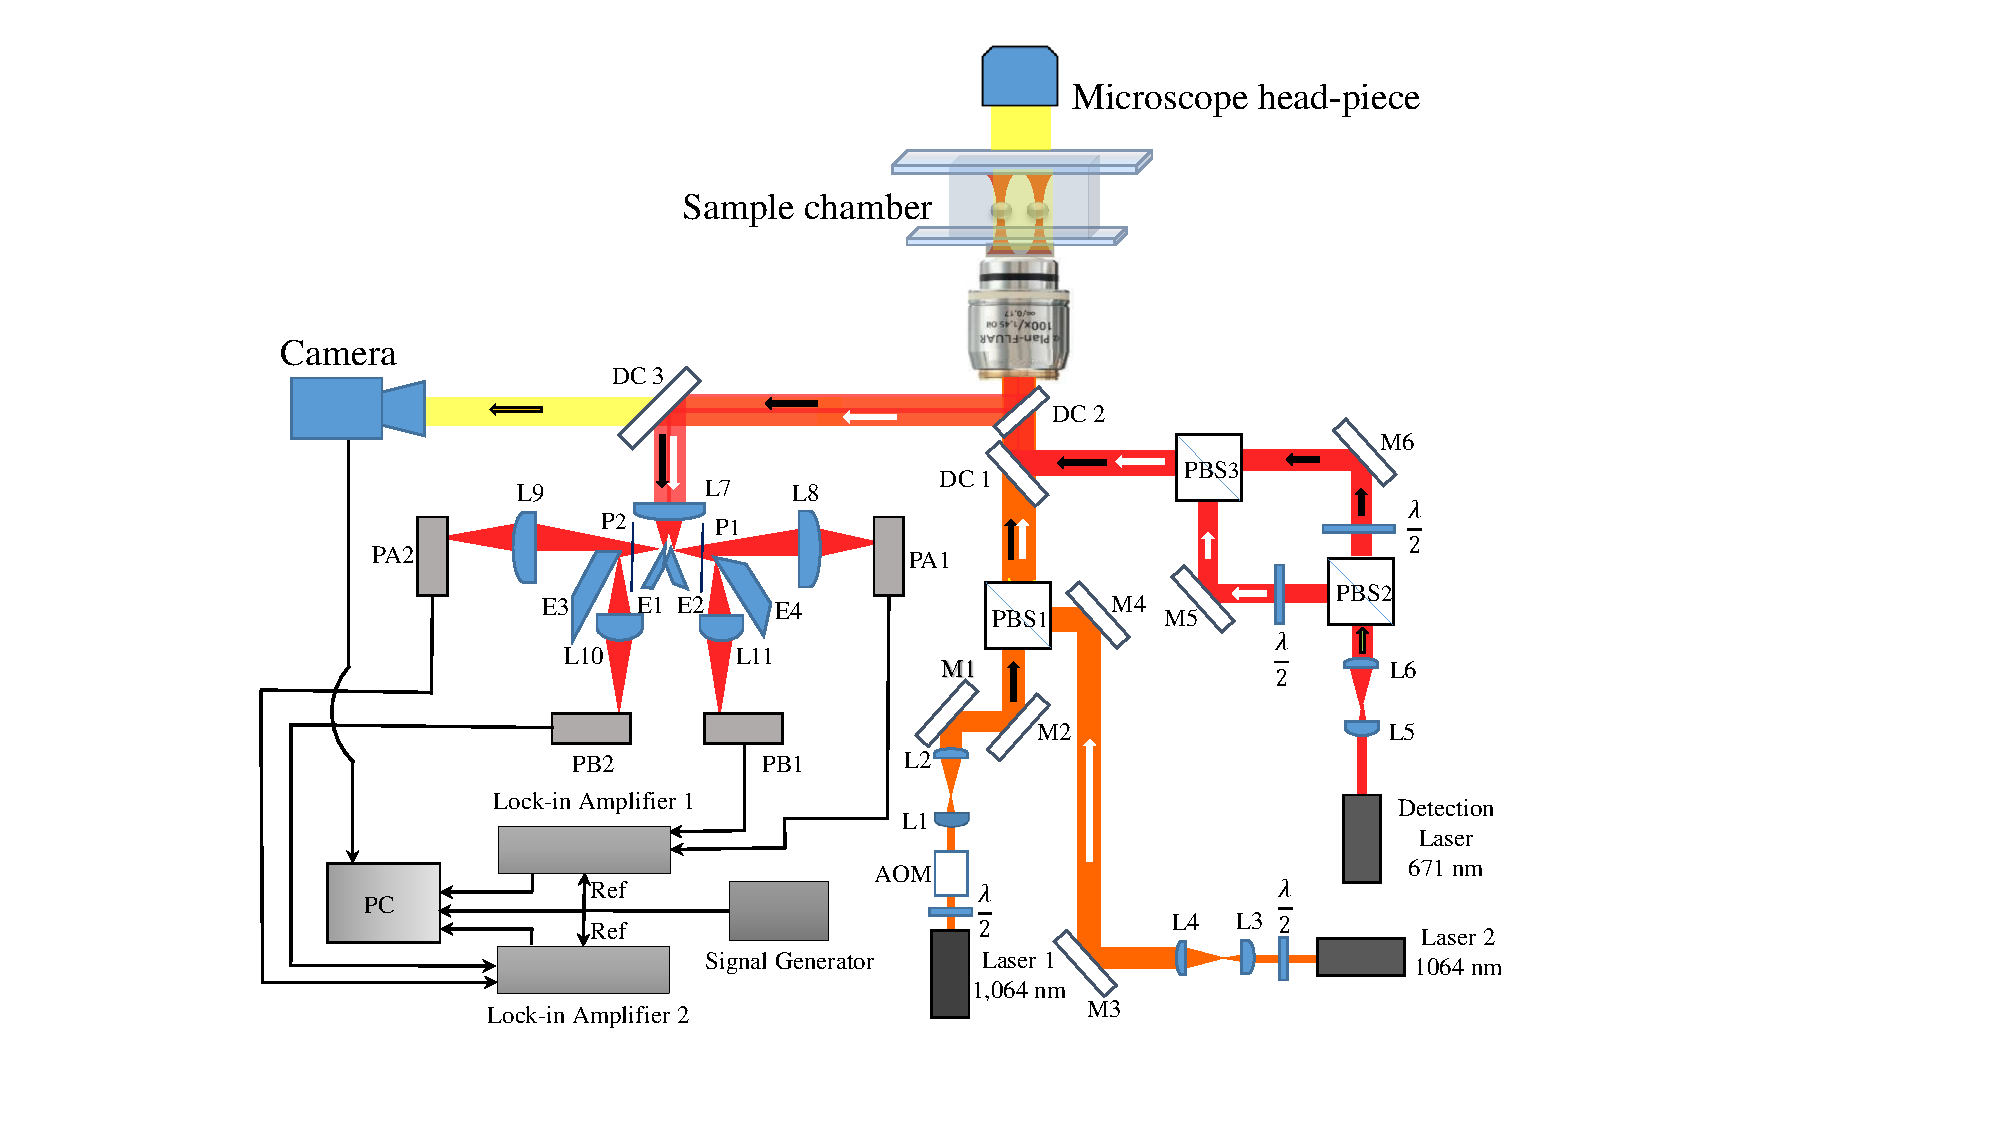
\includegraphics[width=0.45\textwidth]{fig1si} 

\caption{A detailed schematic of the setup is shown. Key:$\frac{\lambda}{2}$:
half-wave plate, L: lens, M: mirror, AOM: accousto optical modulator,
PBS: polarising beam splitter, DC: dicroic mirror respectively, E:
edge mirror, P: polariser, PA, PB: photodiodes. }

\label{Setup} 
\end{figure}

\begin{figure}
\centering 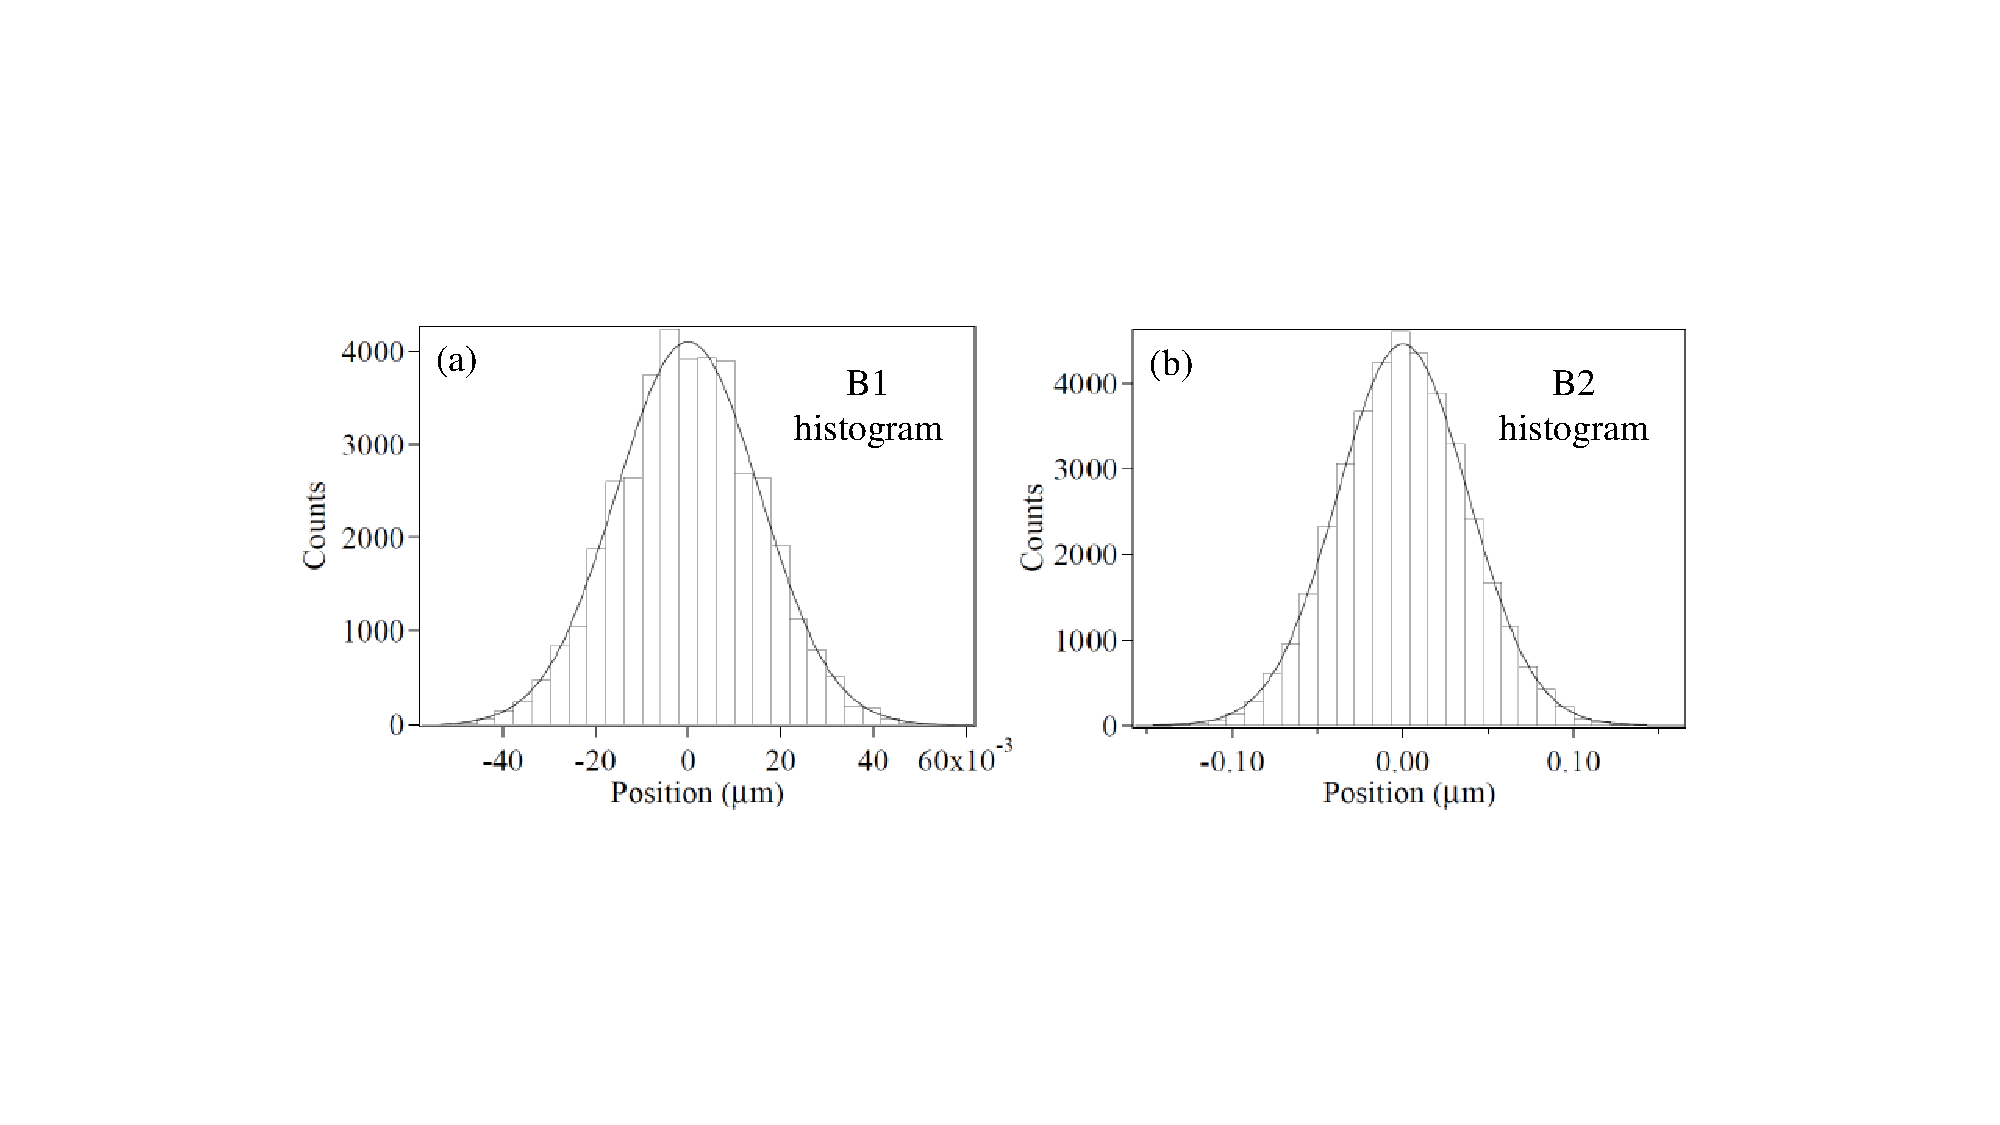
\includegraphics[width=0.45\textwidth]{fig2si} \caption{Position histograms of (a) B1 (driving particle) and (b) B2 (driven
particle). The solid black lines are corresponding Gaussian fits which
show that the potentials are harmonic in nature.}
\label{hist} 
\end{figure}

\begin{figure}
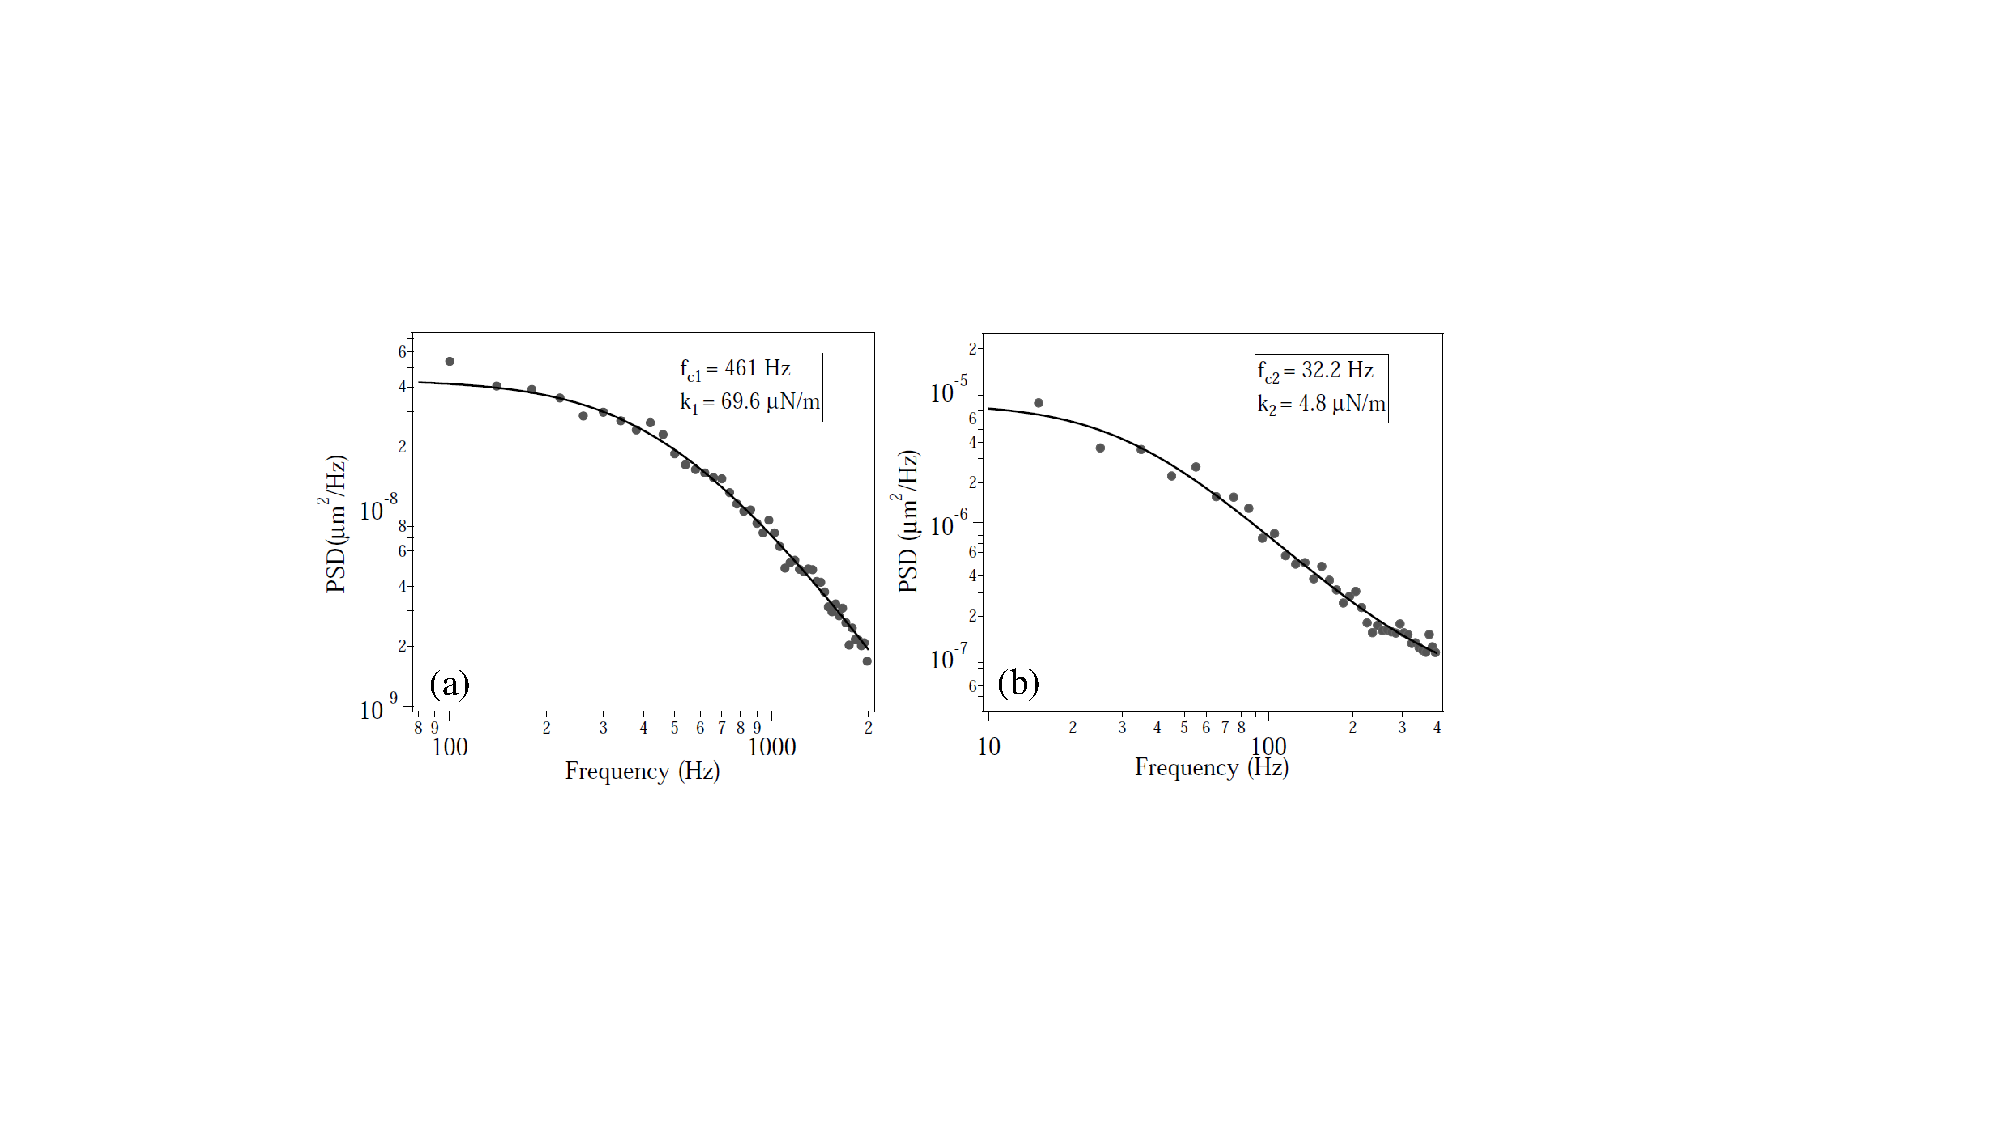
\includegraphics[scale=0.4]{fig3si}\label{psd}\caption{Calibration of traps for B1 and B2. Experimentally measured data points
are shown in filled gray circles, whereas the Lorentzian fit is denoted
by the solid black line. (a) PSD for B1 which has a corner frequency
$\mathit{f_{c1}=\mathrm{461}}$Hz and stiffness $\mathit{k_{1}=\mathrm{69.6}\:\mu}$N/m.
(b) PSD for B2 which has a corner frequency $\mathit{f_{c1}=\mathrm{32.2}}$Hz
and stiffness $\mathit{k_{1}=\mathrm{4.8}\:\mu}$N/m. }
\end{figure}

Fig. \ref{hist} (a) and (b) shows the histogram of position coordinate
data that we acquire for the Brownian motion of driving particle B1
and driven particle B2, respectively. As is clear, the data are normally
distributed in both traps and fit very well to Gaussians (shown in
bold lines). To calibrate the traps and determine the trap stiffnesses,
we measure the power spectral density (PSD) of the Brownian motion
of each particle in the absence of the other. The results are shown
in Fig. \ref{psd}(a) and (b). Each PSD is obtained by data blocking
100 points in the manner described in Ref. \cite{berg2004power}.
The Lorentzian fits to the data are good, and we obtain corner frequencies
$\mathit{f_{c1}}=$461 Hz and $\mathit{f_{c2}}=$32.2 Hz for particles
B1 and B2, which yield stiffnesses of $\mathit{k_{1}=}$69.2 $\mu N/m$
and $\mathit{k_{2}}$= 4.8 $\mu N/m$, respectively. For the two particle
correlation experiments, as a consistency check, we determine the
position cross-correlation function in time domain for B1 and B2 as
shown in Fig. \ref{fig4si}. The data fits well to Eq.5 in Ref. \cite{Meiners99},
with the constant parameters appropriately calculated for our case.
Finally, we demonstrate the amplitude and phase response of the driving
particle B1 as a function of the driving frequency in Fig. \ref{fig5si}(a)
and (b), respectively. As expected, the amplitude decays with increasing
frequency, while the phase is in sync with the drive at low frequencies
and gradually lags behind as the frequency is increased.

\begin{figure}
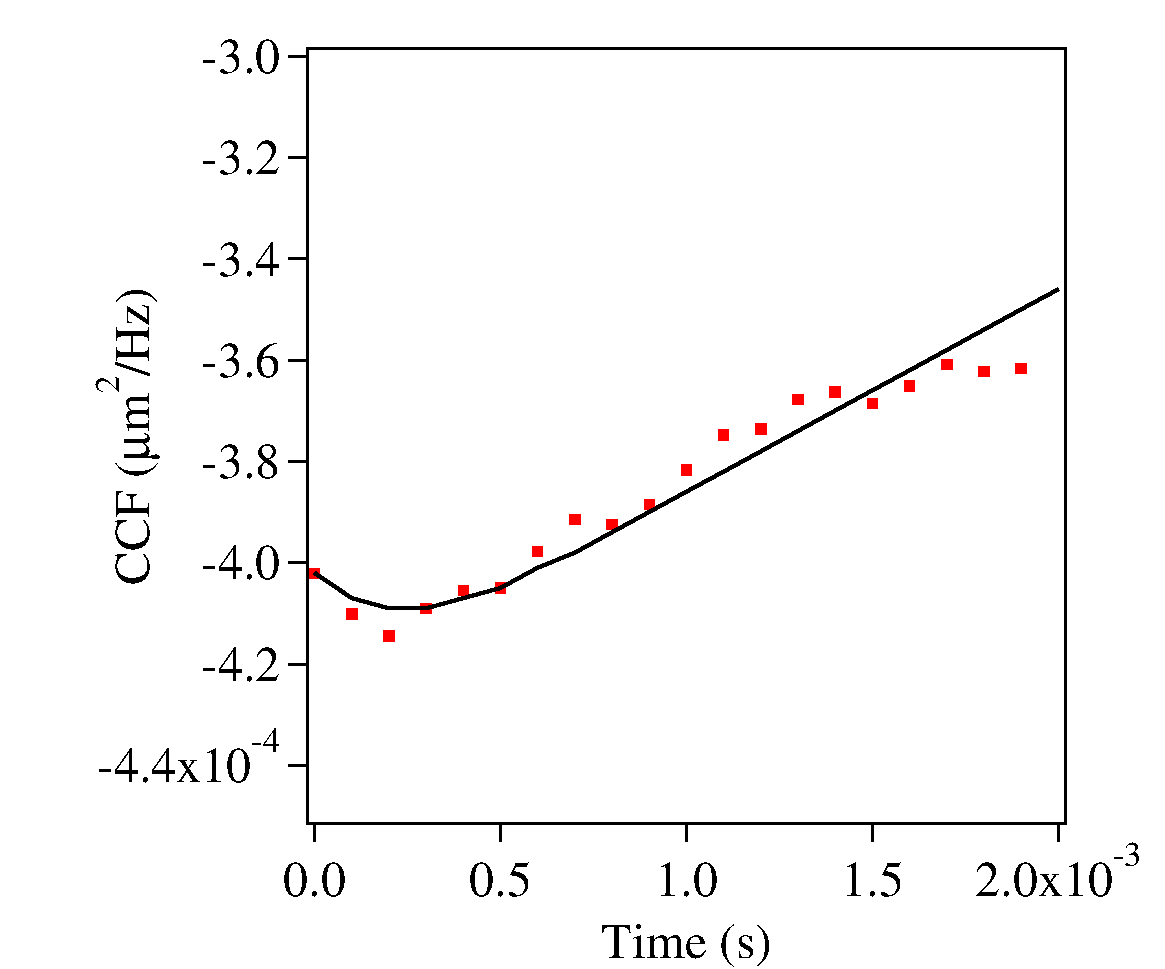
\includegraphics[scale=0.3]{fig4si}\label{fig4si}

\caption{Position cross-correlation in time domain. The filled red squares
are experimentally measured points, while the solid line is the theoretically
calculated cross-correlation.}
\end{figure}

\begin{figure}
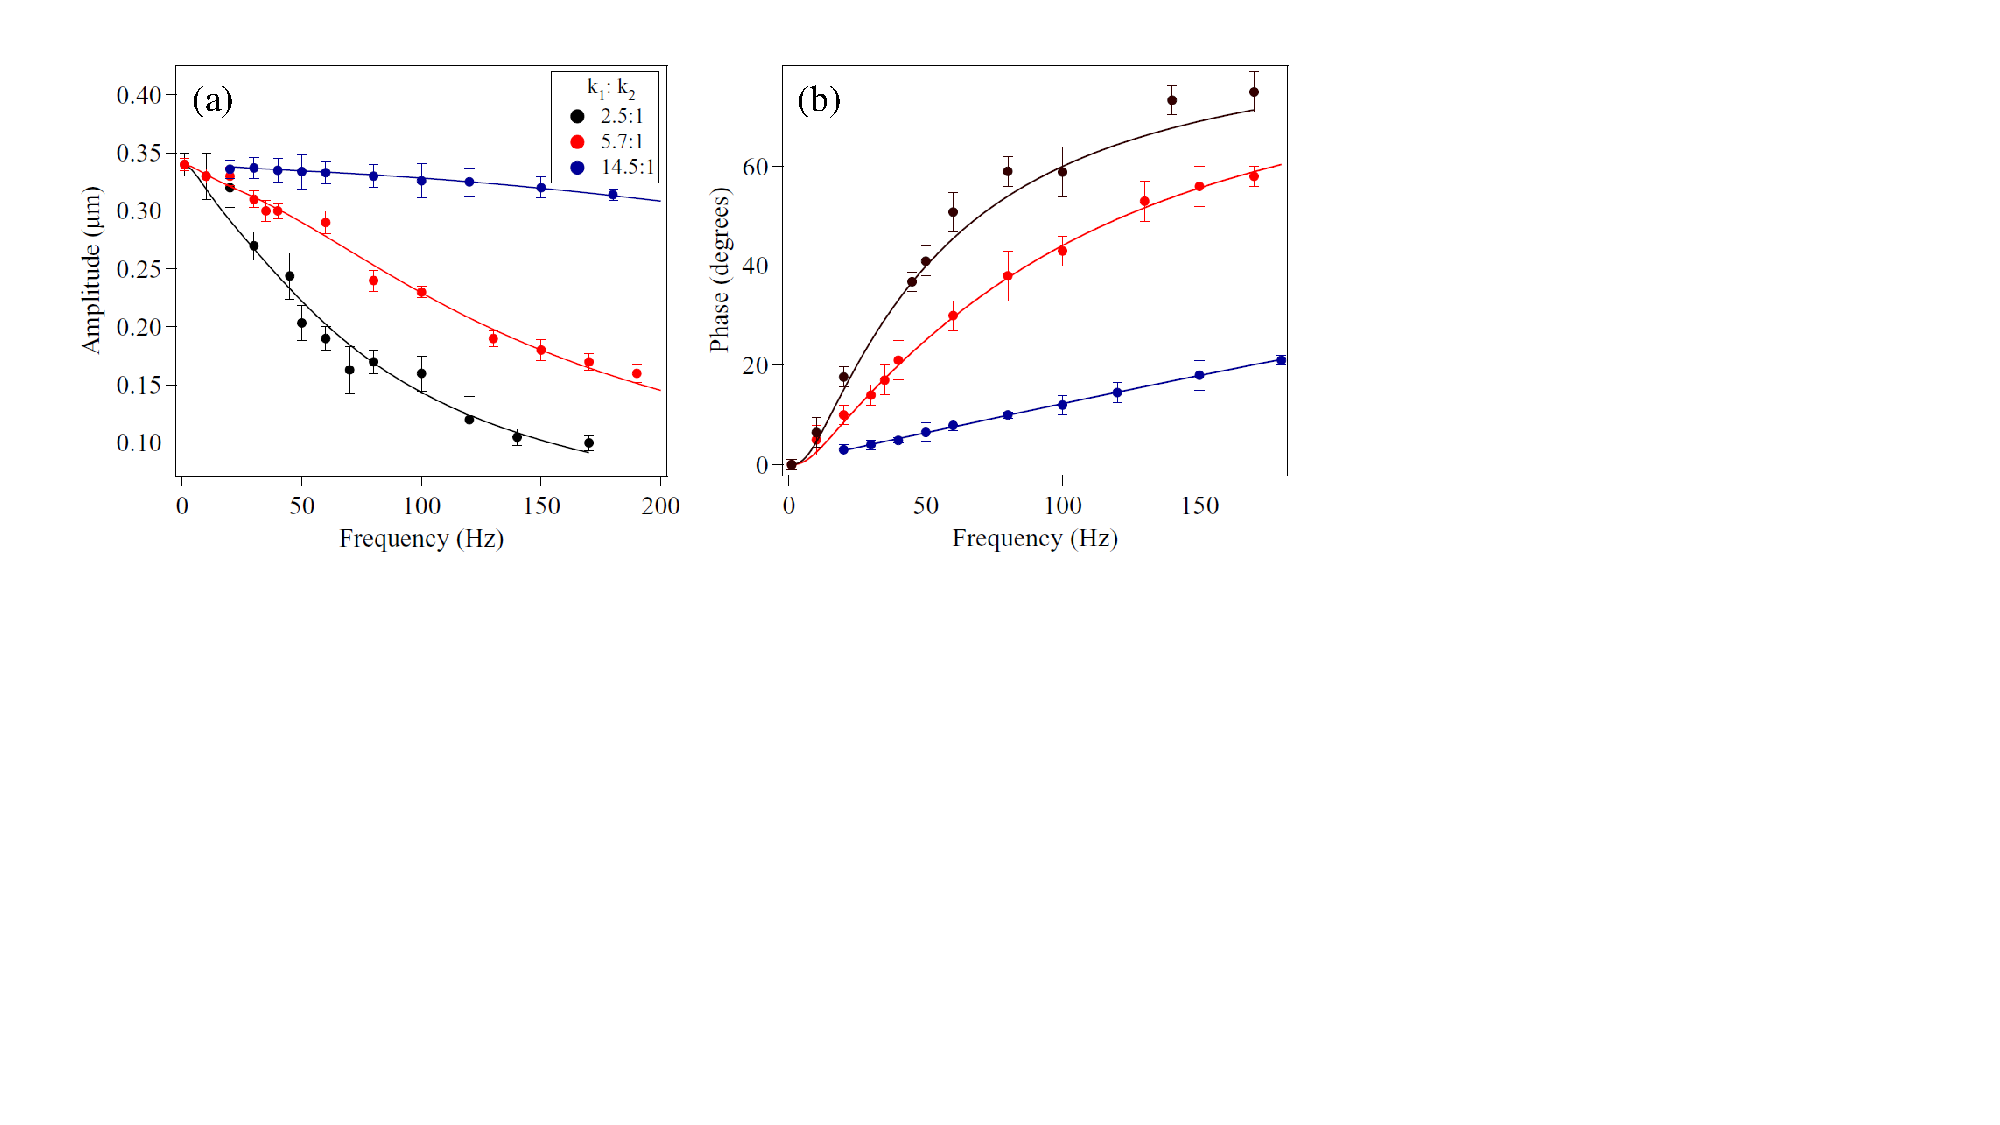
\includegraphics[scale=0.4]{fig5si}

\label{fig5si}\caption{Amplitude (a) and phase (b) response of driving particle B1 as a function
of drive frequency.}
\end{figure}


\section{Theory}

We outline below key steps in deriving the response and correlations
functions on the Smoluchowski time scale, \emph{i.e.} the over-damped
limit, starting from Langevin equations
\begin{align}
m_{i}\dot{\boldsymbol{v}_{i}} & +\boldsymbol{\gamma}_{ij}\cdot\boldsymbol{v}_{j}+{\bf \boldsymbol{\nabla}}_{i}U=\boldsymbol{{\bf \xi}}_{i}\label{eq1}
\end{align}
presented and explained in the main text. 

(\emph{i}) \emph{adiabatic elimination of momentum}: in the first
step, the momenta $m_{i}\boldsymbol{v}_{i}$ are adiabatically eliminated
from the Langevin equations to obtain a contracted description in
terms of the positions alone \cite{gardiner1984adiabatic,gardiner1985handbook}.
This equation is valid on time scales $t\gg m_{i}/\gamma_{i}$. The
heuristic of setting $m_{i}\boldsymbol{v}_{i}$ to zero in the Langevin
equations yields the same result as the more systematic adiabatic
elimination procedure, provided the multiplicative noise is interpreted
correctly and the so-called ``spurious'' drift is included in the
equation for the position increment \cite{van1981ito,van1992stochastic}.
With these caveats, the resulting over-damped Langevin equations are

\begin{equation}
\boldsymbol{\gamma}_{ij}\cdot\boldsymbol{\dot{r}}_{j}+{\bf \boldsymbol{\nabla}}_{i}U=\boldsymbol{{\bf \xi}}_{i}.\label{eq:overdamped}
\end{equation}

(\emph{ii}) \emph{linearization}: in the next step, the equations
are linearized in the small displacements $\boldsymbol{r}_{i}(t)=\boldsymbol{r}_{i}^{0}+\boldsymbol{u}_{i}(t)$,
where $\boldsymbol{r}_{i}^{0}+\boldsymbol{u}_{i}^{0}(t)$ is the \emph{instantaneous}
position of the trap center. The mean distance between the trap centers,
$\boldsymbol{\rho}=\boldsymbol{r}_{1}^{0}-\boldsymbol{r}_{2}^{0}$,
is independent of time. This yields a linear equation of motion for
the small displacements $\boldsymbol{u}_{i}$, where the friction
tensors are now evaluated at the mean separation between the traps.
The linearized Langevin equations are
\begin{equation}
\boldsymbol{\gamma}_{ij}(\boldsymbol{r}_{1}^{0},\boldsymbol{r}_{2}^{0})\cdot\dot{\boldsymbol{u}}_{j}+k_{i}\boldsymbol{u}_{i}-k_{i}\boldsymbol{u}_{i}^{0}(t)=\boldsymbol{\xi}_{i}\label{eq:linearized-LE}
\end{equation}
Note that these are 6 coupled stochastic ordinary differential equations. 

(\emph{iii}) \emph{decoupling through the use of symmetries}: in this
step, the symmetry of the friction tensors under translation, assuming
all boundaries are remote, is used to express them as
\begin{equation}
\boldsymbol{\gamma}_{ij}=\gamma_{ij}^{\parallel}(\rho)\hat{\mathbf{\boldsymbol{\rho}}}\hat{\mathbf{\boldsymbol{\rho}}}+\gamma_{ij}^{\perp}(\rho)(\boldsymbol{I}-\hat{\mathbf{\boldsymbol{\rho}}}\hat{\mathbf{\boldsymbol{\rho}}})\label{eq:gamma-perp-parallel}
\end{equation}
where $\gamma_{ij}^{||}(\rho)$ is the friction coefficient for relative
motion along $\boldsymbol{\rho}$, the line joining the trap centers,
while $\gamma_{ij}^{\perp}(\rho)$ is the corresponding quantity for
motion perpendicular to $\boldsymbol{\rho}$. This motivates the decomposition
of the displacement into components parallel and perpendicular to
$\boldsymbol{\rho},$
\begin{equation}
\boldsymbol{u}_{i}=u_{i}^{\parallel}\hat{\mathbf{\boldsymbol{\rho}}}+\boldsymbol{u}_{i}^{\perp}\cdot(\boldsymbol{I}-\hat{\mathbf{\boldsymbol{\rho}}}\hat{\mathbf{\boldsymbol{\rho}}}).
\end{equation}
Defining the force due to the driving of the trap as $\boldsymbol{f}_{i}(t)=k_{i}\boldsymbol{u}_{i}^{0}(t)$,
averaging the equations over the noise, and using the two previous
equations, we obtain 3 decoupled \emph{pairs} of equations for each
component of motion. For motion along the trap, the pair of coupled
equations is
\begin{equation}
\gamma_{ij}^{||}\dot{u}_{j}^{||}+k_{i}u_{i}^{||}=f_{i}^{||}(t),
\end{equation}
where the dependence of the friction coefficients on relative separation
has been suppressed. The decoupling can be done before the linearization
to give the same result; the two operations commute. 

\emph{(iv}) \emph{response function}: in the final step the coupled
equations are written as
\begin{equation}
\dot{u}_{i}^{||}+A_{ij}u_{j}^{||}=\mu_{ik}^{||}f_{k}
\end{equation}
where $A_{ij}=\mu_{ij}^{||}k_{j}$ is a ``response'' matrix and
the mobility matrix $\mu_{ij}^{||}$ is the inverse of the friction
matrix, $\text{\ensuremath{\gamma_{ik}^{||}\mu_{kj}^{||}}=\ensuremath{\delta_{ij}}}$.
The response function in the frequency domain, then, is \cite{chaikin2000principles}
\begin{equation}
\chi_{ij}^{||}(\omega)=(-i\omega\delta_{ik}+A_{ik})^{-1}\mu_{kj}^{||}.\label{eq:response-function}
\end{equation}
Computing the inverse gives the following expression for the imaginary
part of the response:\begin{widetext}
\begin{align}
\text{Im}\left[\chi_{ij}^{||}(\omega)\right]= & \frac{\omega}{(\text{det}A-\omega^{2})^{2}+(\omega\begin{tabular}{c}
 tr\end{tabular}A)^{2}}\left(\begin{array}{cc}
\begin{tabular}{c}
 \ensuremath{\tfrac{k_{2}}{k_{1}}\mu_{22}^{\parallel}}\end{tabular}\text{det}A+\mu_{11}^{\parallel}\omega^{2} & -\mu_{12}^{\parallel}(\text{det}A-\omega^{2})\\
\, & \,\\
-\mu_{21}^{\parallel}(\text{det}A-\omega^{2}) & \begin{tabular}{c}
 \ensuremath{\tfrac{k_{1}}{k_{2}}\mu_{11}^{\parallel}}\end{tabular}\text{det}A+\mu_{22}\omega^{2}
\end{array}\right).
\end{align}
\end{widetext}The modulus of the response of the first bead to the
driving of the second bead is 
\begin{eqnarray}
|\chi_{21}^{||}| & =\Big| & \frac{i\omega\mu_{21}^{\parallel}}{\text{det}A-\omega^{2}-i\omega\begin{tabular}{c}
 tr\end{tabular}A}\Big|,
\end{eqnarray}
which in non-zero only if there is viscous coupling, $\mu_{12}^{\parallel}\neq0$.
The modulus has a maximum at 
\begin{equation}
\omega_{res}=\sqrt{\text{det}A}=\sqrt{\mu_{11}^{\parallel}\mu_{22}^{\parallel}k_{1}k_{2}\left(1-\frac{\mu_{12}^{\parallel}\mu_{21}^{\parallel}}{\mu_{11}^{\parallel}\mu_{22}^{\parallel}}\right)}.
\end{equation}

\emph{(v}) \emph{correlation function}: To calculate the correlation
function we set the modulation, $\boldsymbol{u}_{i}^{0}(t)$, of the
traps to zero in Eq.(\ref{eq:linearized-LE}) and project, as before,
to obtain the Langevin equation for parallel displacement fluctuations
\begin{gather}
\boldsymbol{\gamma}_{ij}^{\parallel}\dot{u}_{j}^{\parallel}(t)+k_{i}u_{i}^{\parallel}(t)=\xi_{i}^{\parallel}(t),\label{eq:overdamped-1}\\
\langle\xi_{i}^{\parallel}(t)\xi_{j}^{\parallel}(t')\rangle=2k_{B}T\gamma_{ij}^{\parallel}\delta(t-t').
\end{gather}
The Fourier amplitudes of the displacements are
\begin{align}
u_{i}^{\parallel}(\omega) & =(-i\omega\delta_{il}+A_{il})^{-1}\mu_{lk}^{||}\xi_{k}^{\parallel}(\omega),\label{eq:fourier-modes}
\end{align}
and the correlation function is then
\begin{gather}
C_{ij}(\omega)=\langle u_{i}^{\parallel}(\omega)u_{j}^{^{\dagger}\parallel}(\omega)\rangle=\nonumber \\
(-i\omega\delta_{il}+A_{il})^{-1}\mu_{lk}^{||}\langle\xi_{k}\xi_{k'}\rangle\mu_{k'm}^{||}(+i\omega\delta_{mj}+A_{mj}^{T})^{-1}.
\end{gather}
Inserting the variance of the the noise, the correlation function
is\begin{widetext}
\begin{align}
C_{ij}(\omega)= & \frac{2k_{B}T}{(\text{det}A-\omega^{2})^{2}+(\omega\begin{tabular}{c}
 tr\end{tabular}A)^{2}}\left(\begin{array}{cc}
\mu_{22}^{\parallel}k_{2}-i\omega & -\mu_{12}^{\parallel}k_{2}\\
\\
-\mu_{21}^{\parallel}k_{1} & \mu_{11}^{\parallel}k_{1}-i\omega
\end{array}\right)\left(\begin{array}{cc}
\mu_{11}^{\parallel} & \mu_{12}^{\parallel}\\
\\
\mu_{21}^{\parallel} & \mu_{22}^{\parallel}
\end{array}\right)\left(\begin{array}{cc}
\mu_{22}^{\parallel}k_{2}+i\omega & -\mu_{21}^{\parallel}k_{1}\\
\\
-\mu_{12}^{\parallel}k_{2} & \mu_{11}^{\parallel}k_{1}+i\omega
\end{array}\right).
\end{align}
\end{widetext}Completing the matrix multiplications, the final result
is
\begin{align}
C_{ij}(\omega)= & \frac{2k_{B}T}{\omega}\text{Im}\left[\chi_{ij}^{||}(\omega)\right].
\end{align}
This provides an explicit verification of the fluctuation-response
relation for a pair of viscously coupled oscillators \cite{kubo1966fluctuation}.
\bibliographystyle{apsrev4-1}
%\bibliography{2bead-fdt}
%merlin.mbs apsrev4-1.bst 2010-07-25 4.21a (PWD, AO, DPC) hacked
%Control: key (0)
%Control: author (72) initials jnrlst
%Control: editor formatted (1) identically to author
%Control: production of article title (-1) disabled
%Control: page (0) single
%Control: year (1) truncated
%Control: production of eprint (0) enabled
\begin{thebibliography}{9}%
\makeatletter
\providecommand \@ifxundefined [1]{%
 \@ifx{#1\undefined}
}%
\providecommand \@ifnum [1]{%
 \ifnum #1\expandafter \@firstoftwo
 \else \expandafter \@secondoftwo
 \fi
}%
\providecommand \@ifx [1]{%
 \ifx #1\expandafter \@firstoftwo
 \else \expandafter \@secondoftwo
 \fi
}%
\providecommand \natexlab [1]{#1}%
\providecommand \enquote  [1]{``#1''}%
\providecommand \bibnamefont  [1]{#1}%
\providecommand \bibfnamefont [1]{#1}%
\providecommand \citenamefont [1]{#1}%
\providecommand \href@noop [0]{\@secondoftwo}%
\providecommand \href [0]{\begingroup \@sanitize@url \@href}%
\providecommand \@href[1]{\@@startlink{#1}\@@href}%
\providecommand \@@href[1]{\endgroup#1\@@endlink}%
\providecommand \@sanitize@url [0]{\catcode `\\12\catcode `\$12\catcode
  `\&12\catcode `\#12\catcode `\^12\catcode `\_12\catcode `\%12\relax}%
\providecommand \@@startlink[1]{}%
\providecommand \@@endlink[0]{}%
\providecommand \url  [0]{\begingroup\@sanitize@url \@url }%
\providecommand \@url [1]{\endgroup\@href {#1}{\urlprefix }}%
\providecommand \urlprefix  [0]{URL }%
\providecommand \Eprint [0]{\href }%
\providecommand \doibase [0]{http://dx.doi.org/}%
\providecommand \selectlanguage [0]{\@gobble}%
\providecommand \bibinfo  [0]{\@secondoftwo}%
\providecommand \bibfield  [0]{\@secondoftwo}%
\providecommand \translation [1]{[#1]}%
\providecommand \BibitemOpen [0]{}%
\providecommand \bibitemStop [0]{}%
\providecommand \bibitemNoStop [0]{.\EOS\space}%
\providecommand \EOS [0]{\spacefactor3000\relax}%
\providecommand \BibitemShut  [1]{\csname bibitem#1\endcsname}%
\let\auto@bib@innerbib\@empty
%</preamble>
\bibitem [{\citenamefont {Stilgoe}\ \emph {et~al.}(2011)\citenamefont
  {Stilgoe}, \citenamefont {Heckenberg}, \citenamefont {Nieminen},\ and\
  \citenamefont {Rubinsztein-Dunlop}}]{Stilgoe11}%
  \BibitemOpen
  \bibfield  {author} {\bibinfo {author} {\bibfnamefont {A.~B.}\ \bibnamefont
  {Stilgoe}}, \bibinfo {author} {\bibfnamefont {N.~R.}\ \bibnamefont
  {Heckenberg}}, \bibinfo {author} {\bibfnamefont {T.~A.}\ \bibnamefont
  {Nieminen}}, \ and\ \bibinfo {author} {\bibfnamefont {H.}~\bibnamefont
  {Rubinsztein-Dunlop}},\ }\href {\doibase 10.1103/PhysRevLett.107.248101}
  {\bibfield  {journal} {\bibinfo  {journal} {Phys. Rev. Lett.}\ }\textbf
  {\bibinfo {volume} {107}},\ \bibinfo {pages} {248101} (\bibinfo {year}
  {2011})}\BibitemShut {NoStop}%
\bibitem [{\citenamefont {Berg-S{\o}rensen}\ and\ \citenamefont
  {Flyvbjerg}(2004)}]{berg2004power}%
  \BibitemOpen
  \bibfield  {author} {\bibinfo {author} {\bibfnamefont {K.}~\bibnamefont
  {Berg-S{\o}rensen}}\ and\ \bibinfo {author} {\bibfnamefont {H.}~\bibnamefont
  {Flyvbjerg}},\ }\href@noop {} {\bibfield  {journal} {\bibinfo  {journal}
  {Review of Scientific Instruments}\ }\textbf {\bibinfo {volume} {75}},\
  \bibinfo {pages} {594} (\bibinfo {year} {2004})}\BibitemShut {NoStop}%
\bibitem [{\citenamefont {Meiners}\ and\ \citenamefont
  {Quake}(1999)}]{Meiners99}%
  \BibitemOpen
  \bibfield  {author} {\bibinfo {author} {\bibfnamefont {J.-C.}\ \bibnamefont
  {Meiners}}\ and\ \bibinfo {author} {\bibfnamefont {S.~R.}\ \bibnamefont
  {Quake}},\ }\href@noop {} {\bibfield  {journal} {\bibinfo  {journal}
  {Physical Review Letters}\ }\textbf {\bibinfo {volume} {82}},\ \bibinfo
  {pages} {2211} (\bibinfo {year} {1999})}\BibitemShut {NoStop}%
\bibitem [{\citenamefont {Gardiner}(1984)}]{gardiner1984adiabatic}%
  \BibitemOpen
  \bibfield  {author} {\bibinfo {author} {\bibfnamefont {C.~W.}\ \bibnamefont
  {Gardiner}},\ }\href {\doibase 10.1103/PhysRevA.29.2814} {\bibfield
  {journal} {\bibinfo  {journal} {Phys. Rev. A}\ }\textbf {\bibinfo {volume}
  {29}},\ \bibinfo {pages} {2814} (\bibinfo {year} {1984})}\BibitemShut
  {NoStop}%
\bibitem [{\citenamefont {Gardiner}(1985)}]{gardiner1985handbook}%
  \BibitemOpen
  \bibfield  {author} {\bibinfo {author} {\bibfnamefont {C.~W.}\ \bibnamefont
  {Gardiner}},\ }\href@noop {} {\emph {\bibinfo {title} {Handbook of stochastic
  methods}}},\ Vol.~\bibinfo {volume} {3}\ (\bibinfo  {publisher} {Springer
  Berlin},\ \bibinfo {year} {1985})\BibitemShut {NoStop}%
\bibitem [{\citenamefont {van Kampen}(1981)}]{van1981ito}%
  \BibitemOpen
  \bibfield  {author} {\bibinfo {author} {\bibfnamefont {N.~G.}\ \bibnamefont
  {van Kampen}},\ }\href {\doibase 10.1007/BF01007642} {\bibfield  {journal}
  {\bibinfo  {journal} {J. Stat. Phys.}\ }\textbf {\bibinfo {volume} {24}},\
  \bibinfo {pages} {175} (\bibinfo {year} {1981})}\BibitemShut {NoStop}%
\bibitem [{\citenamefont {van Kampen}(1992)}]{van1992stochastic}%
  \BibitemOpen
  \bibfield  {author} {\bibinfo {author} {\bibfnamefont {N.~G.}\ \bibnamefont
  {van Kampen}},\ }\href@noop {} {\emph {\bibinfo {title} {Stochastic processes
  in physics and chemistry}}},\ Vol.~\bibinfo {volume} {1}\ (\bibinfo
  {publisher} {Elsevier},\ \bibinfo {year} {1992})\BibitemShut {NoStop}%
\bibitem [{\citenamefont {Chaikin}\ and\ \citenamefont
  {Lubensky}(2000)}]{chaikin2000principles}%
  \BibitemOpen
  \bibfield  {author} {\bibinfo {author} {\bibfnamefont {P.~M.}\ \bibnamefont
  {Chaikin}}\ and\ \bibinfo {author} {\bibfnamefont {T.~C.}\ \bibnamefont
  {Lubensky}},\ }\href@noop {} {\emph {\bibinfo {title} {Principles of
  condensed matter physics}}},\ Vol.~\bibinfo {volume} {1}\ (\bibinfo
  {publisher} {Cambridge Univ Press},\ \bibinfo {year} {2000})\BibitemShut
  {NoStop}%
\bibitem [{\citenamefont {Kubo}(1966)}]{kubo1966fluctuation}%
  \BibitemOpen
  \bibfield  {author} {\bibinfo {author} {\bibfnamefont {R.}~\bibnamefont
  {Kubo}},\ }\href@noop {} {\bibfield  {journal} {\bibinfo  {journal} {Rep.
  Prog. Phys.}\ }\textbf {\bibinfo {volume} {29}},\ \bibinfo {pages} {255}
  (\bibinfo {year} {1966})}\BibitemShut {NoStop}%
\end{thebibliography}%

\end{document}
